\documentclass[11pt]{article}
\usepackage[a4paper, margin=0.7in]{geometry}
\usepackage{booktabs}
\usepackage{array}
\usepackage{amsmath}
\usepackage{amssymb}
\usepackage{tikz}
\usetikzlibrary{positioning, arrows.meta, shapes.geometric, fit, calc}

\newcolumntype{L}[1]{>{\raggedright\arraybackslash}p{#1}}

\begin{document}

\section*{System Model}

\subsection*{Microgrid Architecture}

\begin{figure}[h!]
\centering
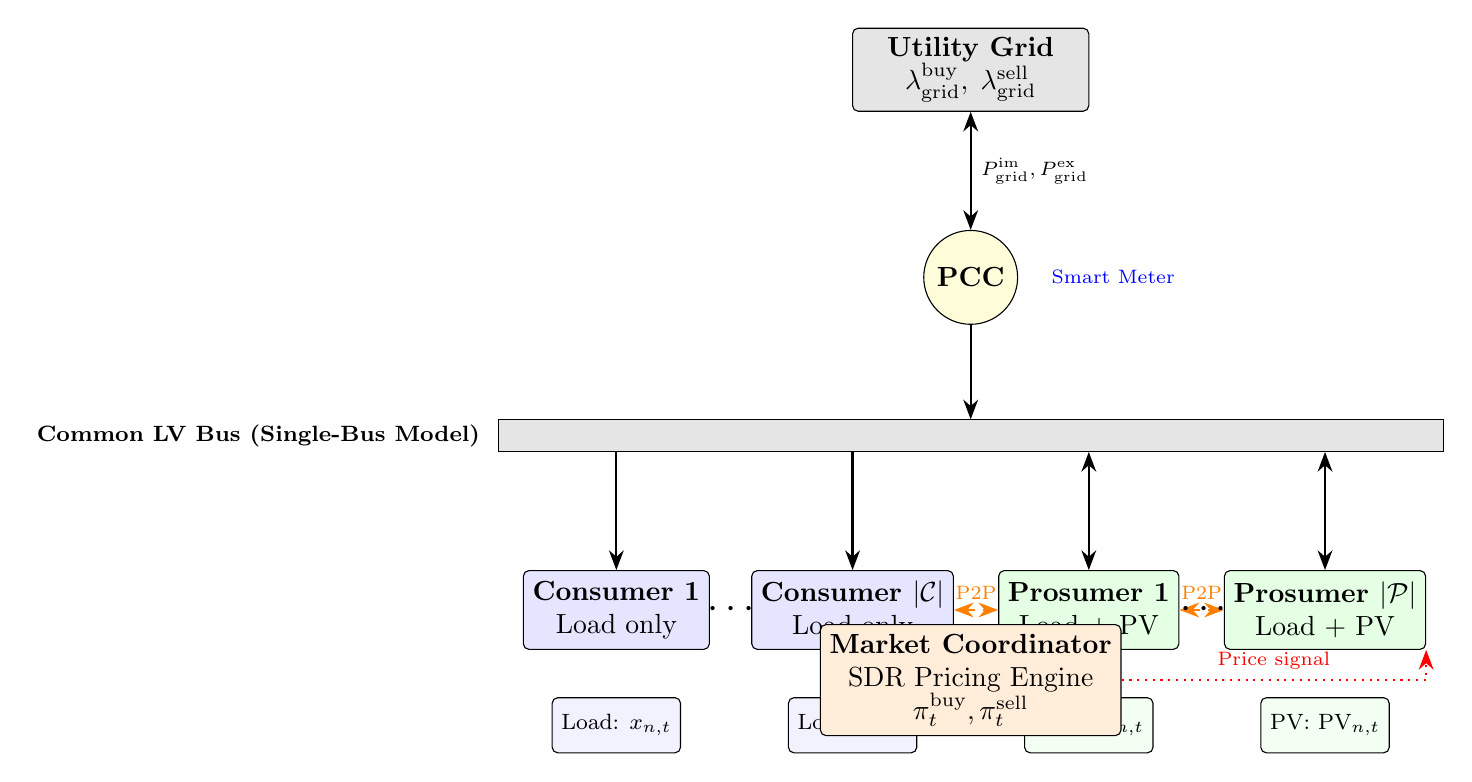
\begin{tikzpicture}[
    node distance=1.2cm and 2cm,
    block/.style={draw, rectangle, minimum width=2.2cm, minimum height=1cm, align=center, rounded corners=2pt},
    smallblock/.style={draw, rectangle, minimum width=1.6cm, minimum height=0.7cm, align=center, font=\footnotesize, rounded corners=2pt},
    arrow/.style={-{Stealth[length=2.5mm]}, thick},
    doublearrow/.style={{Stealth[length=2.5mm]}-{Stealth[length=2.5mm]}, thick},
]

% Utility Grid
\node[block, fill=gray!20, minimum width=3cm] (grid) {\textbf{Utility Grid}\\$\lambda^{\text{buy}}_{\text{grid}},\; \lambda^{\text{sell}}_{\text{grid}}$};

% PCC
\node[below=1.5cm of grid, draw, circle, minimum size=1cm, fill=yellow!15] (pcc) {\textbf{PCC}};

% Common Bus
\node[below=1.2cm of pcc, draw, rectangle, minimum width=12cm, minimum height=0.4cm, fill=black!10] (bus) {};
\node[left=0.1cm of bus, font=\footnotesize\bfseries] {Common LV Bus (Single-Bus Model)};

% Smart Meter at PCC
\node[right=0.3cm of pcc, font=\scriptsize, text=blue] {Smart Meter};

% Households
\node[block, below=1.5cm of bus, xshift=-4.5cm, fill=blue!10] (c1) {\textbf{Consumer 1}\\Load only};
\node[block, below=1.5cm of bus, xshift=-1.5cm, fill=blue!10] (c2) {\textbf{Consumer $|\mathcal{C}|$}\\Load only};
\node[block, below=1.5cm of bus, xshift=1.5cm, fill=green!10] (p1) {\textbf{Prosumer 1}\\Load + PV};
\node[block, below=1.5cm of bus, xshift=4.5cm, fill=green!10] (p2) {\textbf{Prosumer $|\mathcal{P}|$}\\Load + PV};

% Sub-components for prosumer
\node[smallblock, below=0.6cm of p1, fill=green!5] (pv1) {PV: $\text{PV}_{n,t}$};
\node[smallblock, below=0.6cm of p2, fill=green!5] (pv2) {PV: $\text{PV}_{n,t}$};

% Sub-components for consumer
\node[smallblock, below=0.6cm of c1, fill=blue!5] (l1) {Load: $x_{n,t}$};
\node[smallblock, below=0.6cm of c2, fill=blue!5] (l2) {Load: $x_{n,t}$};

% Coordinator / Market
\node[block, below=3.8cm of pcc, fill=orange!15, minimum width=3.5cm] (esp) {\textbf{Market Coordinator}\\SDR Pricing Engine\\$\pi_t^{\text{buy}}, \pi_t^{\text{sell}}$};

% Connections
\draw[doublearrow] (grid) -- node[right, font=\scriptsize] {$P^{\text{im}}_{\text{grid}}, P^{\text{ex}}_{\text{grid}}$} (pcc);
\draw[arrow] (pcc) -- (bus);

\draw[arrow] (bus.south -| c1) -- (c1);
\draw[arrow] (bus.south -| c2) -- (c2);
\draw[doublearrow] (bus.south -| p1) -- (p1);
\draw[doublearrow] (bus.south -| p2) -- (p2);

% P2P arrows
\draw[doublearrow, dashed, color=orange] (p1.east) -- node[above, font=\scriptsize, color=orange] {P2P} (p2.west);
\draw[doublearrow, dashed, color=orange] (c2.east) -- node[above, font=\scriptsize, color=orange] {P2P} (p1.west);

% Price signal
\draw[arrow, dotted, color=red] (esp) -| node[near start, above, font=\scriptsize, color=red] {Price signal} (p2.south east);

% Dots between consumers and prosumers
\node at ($(c1)!0.5!(c2)$) {\Large $\cdots$};
\node at ($(p1)!0.5!(p2)$) {\Large $\cdots$};

\end{tikzpicture}
\caption*{\textbf{Fig. 1:} Single-bus microgrid model. All $N$ households connect to a common LV bus via smart meters. The Point of Common Coupling (PCC) interfaces with the utility grid. P2P energy sharing occurs internally; residual imbalance is settled with the grid at regulated tariffs. The market coordinator computes SDR-based clearing prices each slot.}
\end{figure}

\vspace{0.5cm}

\subsection*{Energy Flow Priority}

\begin{center}
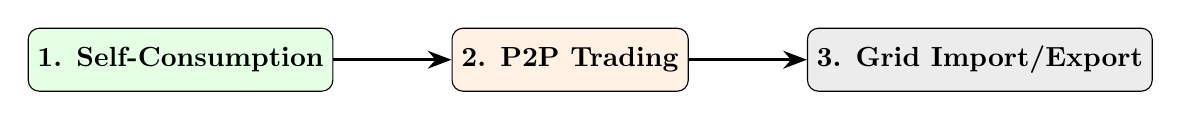
\begin{tikzpicture}[node distance=0.3cm and 1.5cm, arrow/.style={-{Stealth[length=3mm]}, very thick}]
\node[draw, rectangle, rounded corners, fill=green!10, minimum width=3cm, minimum height=0.8cm] (self) {\textbf{1. Self-Consumption}};
\node[draw, rectangle, rounded corners, fill=orange!10, minimum width=3cm, minimum height=0.8cm, right=1.5cm of self] (p2p) {\textbf{2. P2P Trading}};
\node[draw, rectangle, rounded corners, fill=gray!15, minimum width=3cm, minimum height=0.8cm, right=1.5cm of p2p] (gridb) {\textbf{3. Grid Import/Export}};
\draw[arrow] (self) -- (p2p);
\draw[arrow] (p2p) -- (gridb);
\end{tikzpicture}
\end{center}

{\small Each prosumer first consumes own PV generation. Surplus is offered to the P2P market. Only the residual (unmatched P2P demand/supply) interacts with the utility grid.}

\vspace{0.8cm}

%% ASSUMPTIONS
\section*{Simulation Assumptions}

\renewcommand{\arraystretch}{1.4}
\begin{table}[h!]
\centering
\small
\begin{tabular}{L{3.5cm} L{12cm}}
\toprule
\textbf{Category} & \textbf{Assumptions} \\
\midrule

\textbf{1. Network Model} &
\begin{itemize} \setlength\itemsep{0pt}
  \item Single-bus (copper-plate) model --- all households on a common LV bus
  \item Lossless internal power transfer (line losses neglected)
  \item No voltage, thermal, or power flow constraints modeled
  \item Valid for small LV communities where feeder losses $<$2\% [following Liu et al., 2017]
\end{itemize} \\

\textbf{2. Metering \& Communication} &
\begin{itemize} \setlength\itemsep{0pt}
  \item Smart meters at each household with 15-minute resolution ($\Delta t = 0.25$ h)
  \item Instantaneous measurement and reporting --- no communication delays
  \item Perfect metering accuracy (no measurement error modeled)
\end{itemize} \\

\textbf{3. P2P Trading Rules} &
\begin{itemize} \setlength\itemsep{0pt}
  \item Priority: Self-consumption $\rightarrow$ P2P trading $\rightarrow$ Grid interaction
  \item P2P energy allocated proportionally to each participant's surplus/deficit
  \item No transaction fees, network-use charges, or minimum trade volumes
  \item Internal prices bounded: $\pi_{\text{grid}}^{\text{sell}} \leq \pi_t^{\text{int}} \leq \pi_{\text{grid}}^{\text{buy}}$ (no-arbitrage)
\end{itemize} \\

\textbf{4. Market Clearing} &
\begin{itemize} \setlength\itemsep{0pt}
  \item Instantaneous clearing at each time slot (no settlement delays or queuing)
  \item Price-taking behavior --- no strategic bidding or market power
  \item Perfect information: all participants observe the same clearing price
  \item Community power balance: $\sum_n P_{n,t}^{\text{p2p,buy}} = \sum_n P_{n,t}^{\text{p2p,sell}} \;\forall\, t$
\end{itemize} \\

\textbf{5. Load Profiles} &
\begin{itemize} \setlength\itemsep{0pt}
  \item Residential dual-peak load shape (morning $\sim$8:00, evening $\sim$20:00)
  \item Consumer daily load: 4--7 kWh; Prosumer daily load: 5--9 kWh
  \item Day-to-day variability: Gaussian noise ($\sigma = 5$\% daily scaling, 5\% per-slot)
\end{itemize} \\

\textbf{6. PV Generation} &
\begin{itemize} \setlength\itemsep{0pt}
  \item Clear-sky sinusoidal profile (06:00--18:00), peaking at solar noon
  \item PV yield: 4.5--5.5 kWh/kWp/day (typical Indian conditions)
  \item Daily cloud variability: Gaussian ($\sigma = 15$\%)
  \item Consumers have zero PV capacity
\end{itemize} \\

\textbf{7. DSM Constraints} &
\begin{itemize} \setlength\itemsep{0pt}
  \item Load bounds: $D_n^{\text{min}} \leq x_{n,t} \leq D_n^{\text{max}}$ (set at $\pm$50\% of $D_{n,t}^{\text{ref}}$)
  \item Daily energy conservation: $\sum_{t \in d} x_{n,t} \Delta t = \sum_{t \in d} D_{n,t}^{\text{ref}} \Delta t$
  \item Iterative price-response with damping ($\gamma = 0.3$) for convergence
\end{itemize} \\

\textbf{8. Grid Tariffs} &
\begin{itemize} \setlength\itemsep{0pt}
  \item Flat (time-invariant) tariffs: $\lambda^{\text{buy}}_{\text{grid}} = $ Rs 6.0/kWh, $\lambda^{\text{sell}}_{\text{grid}} = $ Rs 3.4/kWh
  \item No time-of-use or dynamic grid pricing
  \item Same buy price for consumers and prosumers
\end{itemize} \\

\textbf{9. Fairness Evaluation} &
\begin{itemize} \setlength\itemsep{0pt}
  \item $\mathcal{F} = 1 - \frac{|s_{\mathcal{C}} - s_{\mathcal{P}}|}{|s_{\mathcal{C}}| + |s_{\mathcal{P}}| + \varepsilon}$ where $s$ = group savings \% vs conventional
  \item Post-hoc metric (not a constraint in the optimization)
  \item $\mathcal{F} = 1$: equal savings for both groups; $\mathcal{F} = 0$: one group gains nothing
\end{itemize} \\

\bottomrule
\end{tabular}
\end{table}

\end{document}
